% cJENguide.tex
% v3.4 released April 2009

\documentclass[]{cJEN2e}


\citestyle{cJEN}
\begin{document}

\doi{10.1080/09544820xxxxxxxxxxxxx}
 \issn{1466-1837} \issnp{0954-4828}
\jvol{00} \jnum{00} \jyear{2009} %\jmonth{October}


\markboth{Taylor \& Francis and I.T. Consultant}{Journal of Engineering Design}

\articletype{GUIDE}

\title{{\itshape Journal of Engineering Design} -- \LaTeXe\ style guide
for authors (Style 2 + References Style V)}

\author{Taylor \& Francis$^{a}$$^{\ast}$\thanks{$^\ast$Corresponding author. Email: latex.helpdesk@tandf.co.uk
\vspace{6pt}} and I.T. Consultant$^{b}$\\\vspace{6pt}  $^{a}${\em{4 Park Square, Milton Park, Abingdon, UK}};
$^{b}${\em{Institut f\"{u}r Informatik, Albert-Ludwigs-Universit\"{a}t, Freiburg,
Germany}}\\\vspace{6pt}\received{v2.3 released April 2009} }

\maketitle

\begin{abstract}
This guide is for authors who are preparing papers for the Taylor \& Francis journal {\em Journal of Engineering Design} ({\it cJEN}\,) using the \LaTeXe\ document preparation system and the Class file {\tt cJEN2e.cls}, which
is available via the journal homepage on the Taylor \& Francis website (see Section~\ref{FTP}). Authors planning
to submit their papers in \LaTeXe\ are advised to use {\tt cJEN2e.cls} as early as possible in the creation of
their files.\bigskip

\begin{keywords}submission instructions; aource file coding;
environments; references citation; fonts {\bf{(Authors: Please provide two to five keywords taken
from terms used in your manuscript}})
\end{keywords}\bigskip

\newpage

\centerline{\bfseries Index to information contained in this
guide}\bigskip
\hbox to \textwidth{\hsize\textwidth\vbox{\hsize24pc
\hspace*{-12pt} {1.}    Introduction\\
\hspace*{7pt} {1.1.}  The {\it cJEN} document style\\
\hspace*{7pt} {1.2.}  Submission of \LaTeXe articles\\
\hspace*{28pt}        to the journal\\
{2.}    Using {\it cJEN} style\\
\hspace*{10pt}{2.1.}  Landscape pages\\
{3.}    Additional features\\
\hspace*{10pt}{3.1.}  Footnotes to article titles\\
\hspace*{28pt}        and authors' names\\
\hspace*{10pt}{3.2.}  Abstracts\\
\hspace*{10pt}{3.3.}  Lists\\
{4.}    Some guidelines for using\\
\hspace*{10pt}        standard features\\
\hspace*{10pt}{4.1.}   Sections\\
\hspace*{10pt}{4.2.}   Illustrations (figures)\\
\hspace*{10pt}{4.3.}   Tables\\
\hspace*{10pt}{4.4.}   Running headlines\\
\hspace*{10pt}{4.5.}   Maths environments\\
\noindent \hspace*{7pt} {4.6.}   Typesetting mathematics\\
\hspace*{24pt} {4.6.1.}   Displayed mathematics\\
\hspace*{24pt} {4.6.2.}  Bold math italic symbols\\
\hspace*{24pt} {4.6.3.}   Bold Greek\\
\hspace*{24pt} {4.6.4.}   Upright Greek characters  \\
\hspace*{7pt} {4.7.}   Acknowledgements \\} \hspace{-84pt}\vbox{\noindent\hsize24pc
\hspace*{7pt} {4.8.}   Notes \\
\hspace*{7pt} {4.9.}   Appendices \\
\hspace*{7pt} {4.10.}   References \\
\hspace*{34pt} {4.10.1.}   References cited in the\\ \hspace*{74pt}text  \\
\hspace*{34pt} {4.10.2.}   The list of references\\
\hspace*{7pt} {4.11.}   {\it cJEN} macros\\
{5.}    Example of a section heading with\\*
\hspace*{10pt}  {\fontencoding{T1}\scshape\lowercase{small caps}},
   \lowercase{lowercase}, {\it italic}, and bold\\*
\hspace*{10pt}  Greek such as
   ${\bm\kappa}$ \\
{6.}   {\em cJEN} journal style \\
\hspace*{10pt}{6.1.}   Punctuation\\
\hspace*{10pt}{6.2.}   Spelling \\
\hspace*{10pt}{6.3.}   Hyphens, n-rules, m-rules and\\ \hspace*{32pt}minus signs\\
\hspace*{10pt}{6.4.}   References \\
\hspace*{10pt}{6.5.}   Maths fonts\\
\noindent   {7.}   Troubleshooting\\
\hspace*{10pt}{7.1.}   Fixes for coding problems\\
     {8.}   Obtaining the cJEN2e Class file\\
\hspace*{10pt}{8.1}  Via the Taylor \& Francis website\\
\hspace*{10pt}{8.2}   Via e-mail\\\\
      }}
\end{abstract}

\noindent{\bf{Please note that the index following the abstract in this guide is provided for information only. An index is not required in submitted papers.}}

\section{Introduction}

All submissions of manuscripts for possible publication in {\itshape Journal of Engineering Design} ({\it cJEN}\,)  should be made online via the journal's Manuscript Central site ({\tt{http://mc.manuscriptcentral.com/cjen}}). New users should first create an account. Once logged on to the site, submissions should be made via the Author Centre. Online user guides and access to a helpdesk are available on this website.

Authors should prepare and upload two versions of their manuscript. One should be a complete text, while in the second all document information identifying the author(s) should be removed from files to allow them to be sent anonymously to referees. When uploading files, authors will then be able to define the non-anonymous version as `File not for review'.

{\it cJEN} accepts papers in any standard format, including Microsoft$\circledR$ Word, PostScript and PDF. Files submitted in formats other than PDF will automatically be converted to a PDF for the review process. \LaTeXe\ files should be converted to PDF prior to submission because Manuscript Central is not able to convert \LaTeXe\ files into PDFs directly. For the submission of manuscripts created using \LaTeXe\, see Section~\ref{S1.2}.

The layout design for {\it cJEN} has been implemented as a \LaTeXe\ Class file. The {\it cJEN} Class file is
based on {\tt article.cls}. Commands that differ from the standard \LaTeXe\ interface, or which are provided in
addition to the standard interface, are explained in this guide. This guide is not a substitute for the \LaTeXe\
manual itself.

This guide can be used as a template for composing an article for submission by cutting, pasting, inserting and
deleting text as appropriate, using the LaTeX environments provided (e.g. \verb"\begin{equation}",
\verb"\begin{corollary}").\vspace{6pt}

\subsection{The {\bi cJEN} document style}

The use of \LaTeXe\ document styles allows a simple change of style (or style option) to transform the appearance
of your document. The cJEN2e Class file preserves the standard \LaTeXe\ interface such that any document that can
be produced using the standard \LaTeXe\ {\tt article} style can also be produced with the {\it cJEN} style.
However, the measure (or width of text) is narrower than the default for {\tt article}, therefore line breaks
will change and long equations may need re-formatting.

When your article appears in the print edition of the {\it gPAV} journal (and exactly reproduced in the PDF
version online), it will have been typeset in Monotype Times. As most authors do not own this font, it is inevitable that the page make-up will change with the change of font. For this reason, we ask authors to ignore details such as slightly long lines, page stretching, or figures falling out of synchronization with their citations in the text, because these details will be dealt with during proofing.

\subsection{Submission of \LaTeXe\ articles to the journal}\label{S1.2}

All submissions of manuscripts for possible publication should be made online via the journal's Manuscript Central site ({\tt{http://mc.manuscriptcentral.com/cjen}}). New users should first create an account. Once logged on to the site, submissions should be made via the Author Centre. Online user guides and access to a helpdesk are available on this website. \LaTeXe\ files should be converted to PDF prior to submission because Manuscript Central is not able to convert \LaTeXe\ files into PDFs directly. The PDF should be uploaded together with the \LaTeXe\ source files and any graphics files.

General Instructions for Authors may be found at
\begin{center}(\nobreak{\tt{http://www.tandf.co.uk/journals/authors/cjenauth.asp}}).\end{center}

Authors should prepare and upload two versions of their manuscript. One should be a complete text, while in the second all document information identifying the author(s) should be removed from files to allow them to be sent anonymously to referees. When uploading files, authors will then be able to define the non-anonymous version as `File not for review'.

Only `open-source' \LaTeXe\ should be used, not proprietary systems such as TCI LaTeX or Scientific WorkPlace. Similarly, Class files such as REVTex4 that produce a document in the style of a different publisher and journal should not be used for preference.

Appropriate gaps should be left for figures, of which original versions and copies should also be supplied.
Authors should ensure that their figures are suitable (in terms of lettering size, etc.) for the reductions they
intend.

Authors who wish to incorporate Encapsulated PostScript artwork directly in their articles can do so by using
Tomas Rokicki's {\tt EPSF} macros (which are supplied with the DVIPS PostScript driver). See Section~\ref{eps},
which also demonstrates how to treat landscape pages. Please remember to supply any additional figure macros you
use with your article in the preamble before \verb"begin{document}". Authors should not attempt to use
implementation-specific \verb"\special"'s directly.

Ensure that any author-defined macros are gathered together in the source file, just before the
\verb"\begin{document}" command.

Please note that, if serious problems are encountered with the coding of a paper (missing author-defined macros,
for example), it may prove necessary to divert the paper to conventional typesetting, i.e. it will be re-keyed.

\section{Using the {\bi cJEN} Class file}

If the file {\tt cJEN2e.cls} is not already in the appropriate system directory for \LaTeXe\ files, either
arrange for it to be put there, or copy it to your working folder. The {\it cJEN} document style is implemented
as a complete document style, {\em not\/} a document style option. In order to use the {\it cJEN} style, replace
{\tt `article'} by {\tt `cJEN2e'} in the \verb"\documentclass" command at the beginning of your document:
%
\begin{verbatim}
\documentclass{article}
\end{verbatim}
%
is replaced by
%
\begin{verbatim}
\documentclass{cJEN2e}
\end{verbatim}
%
In general, the following standard document style options should {\em not\/} be used with the {\it cJEN} style:
%
\begin{enumerate}
   \item {\tt 10pt}, {\tt 11pt}, {\tt 12pt} -- unavailable;
   \item oneside (no associated style file) -- oneside is the default;
   \item {\tt leqno} and {\tt titlepage} -- should not be used;
   \item {\tt singlecolumn} -- is not necessary as it is the default style.
\end{enumerate}
%

\subsection{Landscape pages}\label{eps}

If a table or illustration is too wide to fit the standard measure, it must be turned, with its caption, through
90$^{\circ}$ anticlockwise. Landscape illustrations and/or tables can be produced directly using the cJEN2e style
file using \verb"\usepackage{rotating}" after \verb"\documentclass{cJEN2e}". The following commands can be used
to produce such pages.
%
\begin{verbatim}
\setcounter{figure}{2}
\begin{sidewaysfigure}
\centerline{\epsfbox{fig1.eps}}
\caption{This is an example of figure caption.}
\label{landfig}
\end{sidewaysfigure}
\end{verbatim}
%
\begin{verbatim}
\setcounter{table}{0}
\begin{sidewaystable}
  \tbl{The Largest Optical Telescopes.}
    \begin{tabular}{@{}llllcll}
    .
    .
    .
  \end{tabular}\label{tab1}
\end{sidewaystable}
\end{verbatim}
%
Before any float environment, use the \verb"\setcounter" command
as above to fix the numbering of the caption. Subsequent captions
will then be automatically renumbered accordingly.


\section{Additional features}

In addition to all the standard \LaTeXe\ design elements, {\it cJEN} style includes a separate command for specifying short versions of the authors' names and the journal title for running headlines on the left-hand (verso) and right-hand (recto) pages, respectively (see Section~\ref{markboth}).  In general, once you have used this additional {\tt cJEN2e.cls} feature in your document, do not process it with a standard \LaTeXe\ style file.

\subsection{Footnotes to article titles and authors' names}

On the title page, the \verb"\thanks" control sequence may be used to produce a footnote to either the title or authors' names.

\vspace{6pt}Footnote symbols should be used in the order: $\dagger$
(coded as \verb"\dagger"),\break $\ddagger$ (\verb"\ddagger"), $\S$ (\verb"\S"),
$\P$ (\verb"\P"), $\|$ (\verb"\|"), $\dagger\dagger$
(\verb"\dagger\dagger"),\break $\ddagger\ddagger$
(\verb"\ddagger\ddagger"),  $\S\S$ (\verb"\S\S"), $\P\P$ (\verb"\P\P"),
$\|\|$ (\verb"\|\|").

Note that footnotes to the text will automatically be assigned the superscript
 symbols 1, 2, 3,... by the Class file, beginning afresh on each
page.\footnote{These symbols will be changed to the style of the journal by the
 typesetter during preparation of your proofs.}

The title, author(s) and affiliation(s) should be followed by the {\verb"\maketitle"} command.

\subsection{Abstracts}

At the beginning of your article, the title should be generated in the usual way using the {\verb"\maketitle"}
command. Immediately following the title you should include an abstract. The abstract should be enclosed within
an {\tt abstract} environment. For example, the titles for this guide were produced by the following source code:
%
\begin{verbatim}

\title{{\itshape Journal of Engineering Design} -- \LaTeXe\ style guide %
for authors (Style 2 + References Style V)}

\author{Taylor \& Francis$^{a}$$^{\ast}$\thanks{$^\ast$Corresponding %
author. Email: latex.helpdesk@tandf.co.uk \vspace{6pt}} and I.T. %
Consultant$^{b}$\\\vspace{6pt}  $^{a}${\em{4 Park Square, Milton Park, %
Abingdon, UK}}; $^{b}${\em{Institut f\"{u}r Informatik, %
Albert-Ludwigs-Universit\"{a}t, Freiburg, Germany}}\\\vspace{6pt}%
\received{v2.3 released April 2009} }



\maketitle
\begin{abstract}
This guide is for authors who are preparing papers for the Taylor \& %
Francis journal {\em Journal of Engineering Design} ({\it cJEN}\,) %
using the \LaTeXe\ document preparation system and the Class file %
{\tt cJEN2e.cls}, which is available via the journal homepage on %
the Taylor \& Francis website (see Section~\ref{FTP}). Authors %
planning to submit their papers in \LaTeXe\ are advised to %
use {\tt cJEN2e.cls} as early as possible in the creation of their %
files. \end{abstract}

\end{verbatim}

\noindent{\bf{(Please note that the percentage signs at the ends of lines that quote source code in this document are not part of the coding but have been inserted to achieve line wrapping at the appropriate points.)}}

\subsection{Lists}

The {\it cJEN} style provides numbered and unnumbered lists using the {\tt enumerate} environment and bulleted
lists  using the {\tt itemize} environment.

The enumerated list numbers each list item with arabic numerals:
%
\begin{enumerate}
   \item first item
   \item second item
   \item third item
\end{enumerate}
%
Alternative numbering can be achieved by an argument in square brackets, e.g. \verb"\item[(i)] first item".
%
Unnumbered lists are also provided using the {\tt enumerate} environment.
For example,
\begin{enumerate}
   \item[] First unnumbered indented item without label.
   \item[] Second unnumbered item.
   \item[] Third unnumbered item.
\end{enumerate}
was produced by:
%
\begin{verbatim}
\begin{enumerate}
  \item[] First unnumbered indented item...
  \item[] Second unnumbered item.
  \item[] Third unnumbered item.
\end{enumerate}
\end{verbatim}
%
Bulleted lists are provided using the {\tt itemize} environment. For example,
\begin{itemize}
\item First bulleted item
\item Second bulleted item
\item Third bulleted item
\end{itemize}
was produced by:
\begin{verbatim}
  \begin{itemize}
  \item First bulleted item
  \item Second bulleted item
  \item Third bulleted item
  \end{itemize}
\end{verbatim}


\section[]{Some guidelines for using standard features}

The following notes may help you achieve the best effects with the cJEN2e Class file.

\subsection{Sections}

\LaTeXe\ provides five levels of section headings and they are all defined in the cJEN2e Class file:
\begin{enumerate}
   \item[(A)] \verb"\section"
   \item[(B)] \verb"\subsection"
   \item[(C)] \verb"\subsubsection"
   \item[(D)] \verb"\paragraph"
   \item[(E)] \verb"\subparagraph"
\end{enumerate}
Numbering is automatically generated for section, subsection, subsubsection and paragraph headings.  If you need
additional text styles in the headings, see the examples in Section~5.

\subsection{Illustrations (figures)}

The {\it cJEN} style will cope with most positioning of your illustrations and you should not normally use the
optional positional qualifiers of the {\tt figure} environment, which would override these decisions. See
`Instructions for Authors' in the journal's homepage on the Taylor \& Francis website  for how to submit artwork.
Figure captions should be below the figure itself, therefore the \verb"\caption" command should appear after the
figure. For example, Figure~\ref{sample-figure} with caption and sub-captions is produced using the following
commands:
%
\begin{verbatim}
\begin{figure}
\begin{center}
\vspace{36pt}
\begin{minipage}{100mm}
\subfigure[]{
\resizebox*{5cm}{!}{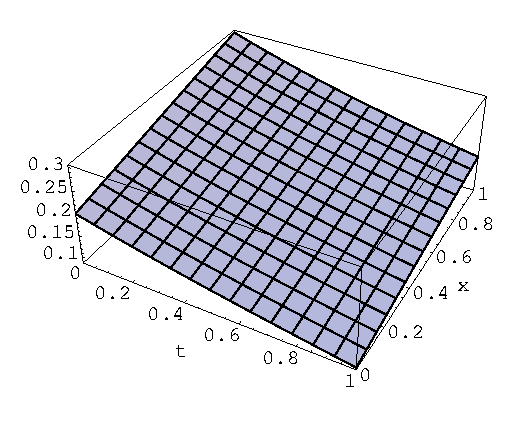
\includegraphics{senu_gr1.eps}}}%
\subfigure[]{
\resizebox*{5cm}{!}{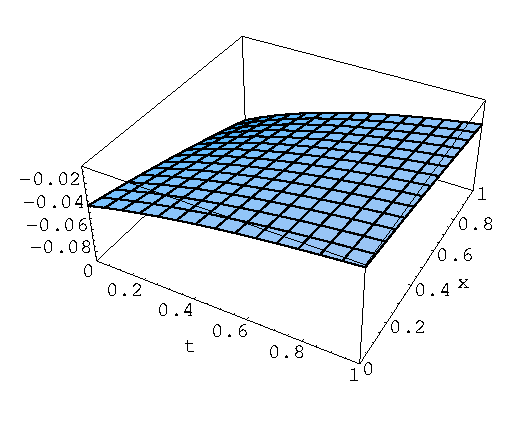
\includegraphics{senu_gr2.eps}}}%
\caption{\label{fig2} Example of a two-part figure with individual %
sub-captions showing that all lines of figure captions range left.}%
\label{sample-figure}
\end{minipage}
\end{center}
\end{figure}
\end{verbatim}

\begin{figure}
\begin{center}
\vspace{36pt}
\begin{minipage}{100mm}
\subfigure[]{
\resizebox*{5cm}{!}{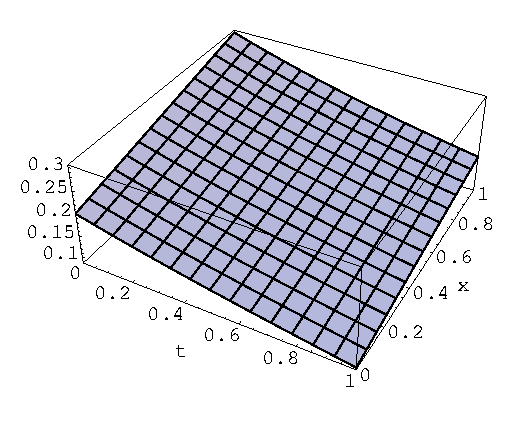
\includegraphics{senu_gr1.eps}}}%
\subfigure[]{
\resizebox*{5cm}{!}{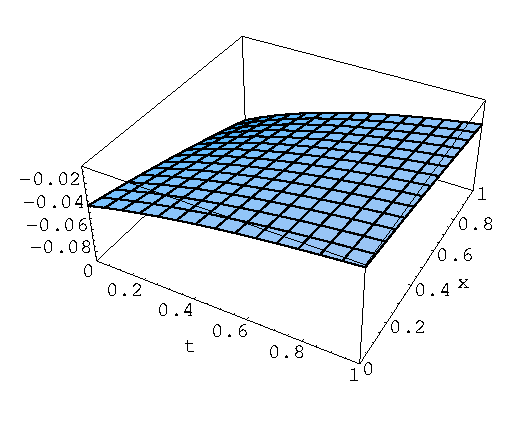
\includegraphics{senu_gr2.eps}}}%
\caption{Example of a two-part figure with individual %
sub-captions showing that all lines of figure captions range left.}%
\label{sample-figure}
\end{minipage}
\end{center}
\end{figure}

The control sequences \verb"\epsfig{}", \verb"\subfigure{}" and \verb"\includegraphics{}" require epsfig.sty,
subfigure.sty and graphicx.sty. These are called by the Class file cJEN2e.cls and are included with the LaTeX
package for this journal for convenience.

To ensure that figures are correctly numbered automatically, the \verb"\label{}" command should be inserted just
after \verb"\caption{}"


\subsection{Tables}

The {\it cJEN} style will cope with most positioning of your tables and you should not normally use the optional
positional qualifiers of the {\tt table} environment, which would override these decisions. The table caption
appears above the body of the table in {\it cJEN} style, therefore the \verb"\tbl" command should appear before
the body of the table.

The {\tt tabular} environment can be used to produce tables with single thick and thin horizontal rules, which
are allowed, if desired. Thick rules should be used at the head and foot only and thin rules elsewhere.

Commands to redefine quantities such as \verb"\arraystretch" should be omitted. For example, Table~\ref{symbols}
is produced using the following commands. Note that \verb"\rm" will produce a roman character in math mode. There
are also \verb"\bf" and \verb"\it", which produce bold face and text italic in math mode.

\begin{table}
\vspace{36pt}
  \tbl{Radio-band beaming model parameters for {FSRQs and BL Lacs.}}
{\begin{tabular}[l]{@{}lcccccc}\toprule
   Class$^{\rm a}$
  & $\gamma _1$ & $\gamma _2$$^{\rm b}$
         & $\langle \gamma \rangle$
         & $G$ & $|{\bm f}|$ & $\theta _{c}$ \\
\colrule
   BL Lacs &5 & 36 & 7 & $-4.0$
         & $1.0\times 10^{-2}$ & 10$^\circ$ \\
   FSRQs & 5 & 40 & 11 & $-2.3$
         & $0.5\times 10^{-2}$ & 14$^\circ$ \\
   \botrule
  \end{tabular}}
\tabnote{$^{\rm a}$This footnote shows what footnote symbols to use.\\$^{\rm b}$This footnote shows the
text turning over when necessary.}\label{symbols}
\end{table}


\begin{verbatim}
\begin{table}
\vspace{36pt}
  \tbl{Radio-band beaming model parameters
           for {FSRQs and BL Lacs.}}
{\begin{tabular}{@{}lcccccc}\toprule
   Class$^{\rm a}$
  & $\gamma _1$ & $\gamma _2$$^{\rm b}$
         & $\langle \gamma \rangle$
         & $G$ & $|{\bm f}|$ & $\theta _{c}$ \\
\colrule
   BL Lacs &5 & 36 & 7 & $-4.0$
         & $1.0\times 10^{-2}$ & 10$^\circ$ \\
   FSRQs & 5 & 40 & 11 & $-2.3$
         & $0.5\times 10^{-2}$ & 14$^\circ$ \\
   \botrule
  \end{tabular}}
\tabnote{$^{\rm a}$This footnote shows what footnote symbols to
use.\\$^{\rm b}$This footnote shows the text turning over when %
necessary.}\label{symbols}
\end{table}
\end{verbatim}

To ensure that tables are correctly numbered automatically, the
\verb"\label{}" command should be inserted just before
\verb"\end{table}".

\subsection{Running headlines}\label{markboth}

As described above, the title of the journal or the author's name (or authors' names) are used as running headlines at the top of every page. The headline on left-hand pages can list up to two names; for more than two use {\it et~al.} The \verb"\pagestyle" and \verb"\thispagestyle" commands should {\it not\/} be used.

\subsection{Maths environments}

The {\it cJEN} style provides for the following maths environments.

\begin{lemma}
More recent algorithms for solving the semidefinite programming
relaxation are particularly efficient, because they explore the structure
of the MAX-CUT.
\end{lemma}
\begin{theorem}
More recent algorithms for solving the semidefinite programming
relaxation are particularly efficient, because they explore the structure
of the MAX-CUT.
\end{theorem}
\begin{corollary}
More recent algorithms for solving the semidefinite programming
relaxation are particularly efficient, because they explore the
structure of the MAX-CUT.
\end{corollary}
\begin{proposition}
More recent algorithms for solving the semidefinite programming
relaxation are particularly efficient, because they explore the structure
of the MAX-CUT.
\end{proposition}
\begin{proof}
More recent algorithms for solving the semidefinite programming
relaxation are particularly efficient, because they explore the structure
of the MAX-CUT.
\end{proof}
\begin{remark}
More recent algorithms for solving the semidefinite programming
relaxation are particularly efficient, because they explore the
structure of the MAX-CUT problem.
\end{remark}
\begin{algorithm}
More recent algorithms for solving the semidefinite programming
relaxation are particularly efficient, because they explore the
structure of the MAX-CUT problem.
\end{algorithm}

\noindent These were produced by:
\begin{verbatim}
\begin{lemma}
More recent algorithms for solving the semidefinite
programming relaxation are particularly efficient,
because they explore the structure of the MAX-CUT.
\end{lemma}

\begin{theorem}
...
...
\end{theorem}

\begin{corollary}
...
...
\end{corollary}

\begin{proposition}
...
...
\end{proposition}

\begin{proof}
...
...
\end{proof}

\begin{remark}
...
...
\end{remark}

\begin{algorithm}
...
...
\end{algorithm}

\end{verbatim}


\subsection{Typesetting mathematics}\label{TMth}

\subsubsection{Displayed mathematics}

The {\it cJEN} style will set displayed mathematics centred on the measure without equation numbers, provided
that you use the \LaTeXe\ standard control sequences open (\verb"\[") and close (\verb"\]") square brackets as
delimiters. The equation
\[
  \sum_{i=1}^p \lambda_i = {\rm trace}({\textrm{\bf S}})\qquad
  i\in {\mathbb R}
\]
\normalfont was typeset in the {\it cJEN} style using the commands
%
\begin{verbatim}
\[
  \sum_{i=1}^p \lambda_i = {\rm trace}({\textrm{\bf S}})\qquad
  i\in {\mathbb R}
\].
\end{verbatim}

For those of your equations that you wish to be automatically
numbered sequentially throughout the text, use the {\tt{equation}}
environment, e.g.

\begin{equation}
  \sum_{i=1}^p \lambda_i = {\rm trace}({\textrm{\bf S}})\qquad
  i\in {\mathbb R}
\end{equation}

was typeset using the commands

\begin{verbatim}
\begin{equation}
  \sum_{i=1}^p \lambda_i = {\rm trace}({\textrm{\bf S}})quad
  i\in {\mathbb R}
\end{equation}
\end{verbatim}

Part numbers for sets of equations may be generated using the
{\tt{subequations}} environment, e.g.
\begin{subequations} \label{subeqnexample}
\begin{equation}
        \varepsilon \rho w_{tt}(s,t)
        =
        N[w_{s}(s,t),w_{st}(s,t)]_{s},
        \label{subeqnpart}
\end{equation}
\begin{equation}
        w_{tt}(1,t)+N[w_{s}(1,t),w_{st}(1,t)] = 0,
\end{equation}
\end{subequations}
which was generated using the control sequences

\begin{verbatim}
\begin{subequations} \label{subeqnexample}
\begin{equation}
        \varepsilon \rho w_{tt}(s,t)
        =
        N[w_{s}(s,t),w_{st}(s,t)]_{s},
        \label{subeqnpart}
\end{equation}
\begin{equation}
        w_{tt}(1,t)+N[w_{s}(1,t),w_{st}(1,t)] = 0,
\end{equation}
\end{subequations}
\end{verbatim}
This is made possible by the package {\tt{subeqn}}, which is called
by the Class file. If you put the \verb"\label{}" just after the
\verb"\begin{subequations}" line, references will be to the
collection of equations, `(\ref{subeqnexample})' in the example
above. Or, like the example code above, you can reference each
equation individually -- e.g. `(\ref{subeqnpart})'.

\subsubsection{Bold math italic symbols}

To get bold math italic you can use \verb"\bm", which works for
all sizes, e.g.
%
\begin{verbatim}
\sffamily
\begin{equation}
   {\rm d}({\bm s_{t_{\bm u}}) = \langle{\bm\alpha({\sf{\textbf L}})}%
   [RM({\bm X}_y + {\bm s}_t) - RM({\bm x}_y)]^2 \rangle.
\end{equation}
\normalfont
\end{verbatim}
%
produces\sffamily
\begin{equation}
   {\rm d}({\bm s_{t_{\bm u}}}) = \langle {\bm\alpha({\sf{\textbf L}})}[RM({\bm X}_y
   + {\bm s}_t) - RM({\bm x}_y)]^2 \rangle.
\end{equation}\normalfont
Note that subscript, superscript, subscript to subscript, etc.
sizes will take care of themselves and are italic, not bold,
unless coded individually. \verb"\bm" produces the same effect as
\verb"\boldmath". \verb"\sffamily"...\verb"\normalfont" allows
upright sans serif fonts to be created in math mode by using the
control sequence `\verb"\sf"'.



\subsubsection{Bold Greek}\label{boldgreek}

Bold lowercase as well as uppercase Greek characters can be
obtained by \verb"{\bm \gamma}", which gives ${\bm \gamma}$, and
\verb"{\bm \Gamma}", which gives ${\bm \Gamma}$.


\subsubsection{Upright lowercase Greek characters and the upright partial derivative sign}\label{upgreek}

Upright lowercase Greek characters can be obtained with the Class file by inserting the letter `u' in the control
code for the character, e.g. \verb"\umu" and \verb"\upi" produce $\umu$ (used, for example, in the symbol for the
unit microns -- $\umu{\rm m}$) and $\upi$ (the ratio of the circumference to the diameter of a circle). Similarly,
the control code for the upright partial derivative $\upartial$ is \verb"\upartial".

\subsection{Acknowledgements}

This unnumbered section, e.g. \verb"\section*{Acknowledgement(s)}", should be used for thanks, grant details, etc.
and placed before any Notes or References sections.

\subsection{Notes}

This unnumbered section, e.g. \verb"\section*{Note(s)}", may be placed before any References section.

\subsection{Appendices}

Appendices should be set after the references, beginning with the
command \verb"\appendices" followed by the command \verb"\section"
for each appendix title, e.g.
%
\begin{verbatim}
\appendices
\section{This is the title of the first appendix}
\section{This is the title of the second appendix}
\end{verbatim}

\noindent produces\medskip

\noindent Appendix A. This is the title of the first appendix

\noindent Appendix B. This is the title of the second appendix

\medskip
Subsections, equations, theorems, figures, tables, etc. within
appendices will then be automatically numbered as appropriate.


\subsection{References}\label{refs}

\subsubsection{References cited in the text} References should be cited in the text in  author--date (Harvard) style -- e.g. `(Smith 1985, Jones 1986, Trevor and Atkins 1987, Bloggs {\itshape{et al.}} 2001)' or `\ldots\,\, see Smith (1985, p. 75) \ldots' (note that these references have been cited in chronological order and `{\itshape{et al.}}' has been used where a reference has three or more authors). If two or more references by the same author(s) published in the same year are cited, distinguish these by adding a,b,c, etc. after the year, e.g. `Johnson (1994a) discussed \ldots' If a source is quoted in another source, cite both in the text, but only list the work you read in the bibliography: `A study by Smith (1960 cited Jones 1994) showed that \ldots'

References should be listed in the references section at the end of the main text in alphabetical order, then chronologically (earliest first), with both issue numbers and full page ranges for journals where appropriate. If a reference has four or more authors, quote only the first followed  by `{\itshape{et al.}}' A smaller font than in the main body text should be used, with a hanging indent. Each bibliographical entry has a key, which is assigned by the author and used to refer to that entry in the text. In this document, the key \verb"ev94" in the citation form \verb"\citep{ev94}" produces `\citep{ev94}', and the keys \verb"ev94", \verb"GloRib51", \verb"PeaEtAl76" and \verb"Holl04" in the citation form \verb"\citep{ev94,PeaEtAl76,Holl04,GloRib51}" produce `\citep{ev94,PeaEtAl76,Holl04,GloRib51}'. The appropriate citation style in the text for different situations can be produced by \verb"\citet{fzf88}" for `\citet{fzf88}', \verb"\citealt{Kor95}" for `\citealt{Kor95}' and `\verb"\citet{fwp02,cww86,cwm73,fzf88}" and \verb"\citet{hk97}"' for `\citet{fwp02,cww86,cwm73,fzf88} and \citet{hk97}'. Optional notes may be included at the beginning and end of a citation by the use of square brackets, e.g. \verb"\citep[see][and" \verb"references" \verb"therein]{Agu95}" produces `\citep[see][and references therein]{Agu95}'. Citation of the year alone may be produced by \verb"\citeyear{PeaEtAl76}", i.e. `\citeyear{PeaEtAl76}', or \verb"\citeyearpar{PeaEtAl76}", i.e. `\citeyearpar{PeaEtAl76}'.

\subsubsection{The list of references} The following listing shows some references prepared in the style of the
journal; note that references with four or more authors begin with the first-named author's initials and
surname followed by `{\em{et~al.}}'; references having the same author(s) are listed chronologically, beginning with the earliest.
%
%
\begin{thebibliography}{9}

\markboth{Taylor \& Francis and I.T. Consultant}{Journal of Engineering Design}

\bibitem[\protect\citeauthoryear{Agutter}{1995}]{Agu95}
Agutter, A.J., 1995. The linguistic significance of current British slang.
  Thesis (PhD). Edinburgh University, UK.

\bibitem[\protect\citeauthoryear{Cutler {\itshape{et~al.}}}{1986}]{cww86}
Cutler, T., Williams, K., and Williams, J., 1986. {\itshape Keynes, Beveridge and
  beyond}. 3rd ed. Twentieth century political economics Vol. II. London:
  Routledge.

\bibitem[\protect\citeauthoryear{Evans}{1994}]{ev94}
Evans, W.A., 1994. Approaches to intelligent information retrieval. {\itshape
  Information Processing and Management}, 7 (2), 147--168.

\bibitem[\protect\citeauthoryear{French}{1988}]{fzf88}
French, F., 1988. English title of a chapter in the translation of a book in a
  foreign language.  {\itshape{In}}: {\itshape Title of a book in another language (Quoted in
  that language)}  [{\itshape English translation}],  translated by P. Smith.
  New York: Dover (original work published 1923).

\bibitem[\protect\citeauthoryear{Glover and Ribeiro}{1951}]{GloRib51}
Glover, F. and Ribeiro, C.C., eds, 1951. {\itshape
Lessons of the British war economy}. 2nd ed. Westport, CT: Greenwood Press, 1--24.

\bibitem[\protect\citeauthoryear{Holland}{2004}]{Holl04}
Holland, M., 2004. {\itshape Guide to citing Internet sources} [online]. Poole, UK: Bournmouth University. Available from:
  http://www.bournemouth.ac.uk/library/using/guide\_to\_citing\_internet\_sourc.%
  html [Accessed 4 November 2004].

\bibitem[\protect\citeauthoryear{Kern}{1997}]{hk97}
Kern, H., 1997. The resurgent Japanese economy and a Japan--United States free trade
  agreement. {\itshape {In}}: C.~Lambert and G.~Holst, eds. {\itshape 4th international conference on the restructuring of the economic and political system in Japan}, Milan, Italy, 21--25 May 1996. Singapore: World Scientific, 147--156.

\bibitem[\protect\citeauthoryear{Korb}{1995}]{Kor95}
Korb, K.B., 1995. Persons and things: book review of Bringsjord on
  robot-consciousness. {\itshape Psycoloquy} [online], 6 (15). Available from: http://psycprints.ecs.soton.ac.uk/archive/00000462/ [Accessed 20 May 2004].

\bibitem[\protect\citeauthoryear{Misner}{1973}]{cwm73}
Misner, C.W., ed., 1973. Efficient algorithms for layer assignment problems. {\itshape{In}}:
  {\itshape Gravitation in a collapsing Universe}. San Francisco, CA:
  Freeman.

\bibitem[\protect\citeauthoryear{Patel}{2002}]{fwp02}
Patel, F.W., 2002. {\itshape Banking technology in an age of cynicism}. Mongraphs on
  technical aspects Vol. XIII. New York: Dover.

\bibitem[\protect\citeauthoryear{Pierce {\itshape{et~al.}}}{1976}]{PeaEtAl76}
Pierce, I.F., {\itshape{et al.}}, 1976. A
  model of output, employment, wages and prices in the UK. {\itshape{In}}: M.~Laguna and
  J.L. Gonz\'{a}les-Velarde, eds. {\itshape Computing tools for modeling, optimization and simulation: interfaces in
  computer science and operations research}. 2nd  ed. Boston, MA: Cambridge University
  Press, 1--24.
\end{thebibliography}
\markboth{Taylor \& Francis and I.T. Consultant}{Journal of Engineering Design}
\medskip
\noindent This list was produced by:
\medskip

\begin{verbatim}
\begin{thebibliography}

\bibitem[\protect\citeauthoryear{Agutter}{1995}]{Agu95}
Agutter, A.J., 1995. The linguistic significance of current British %
slang. Thesis (PhD). Edinburgh University, UK.

\bibitem[\protect\citeauthoryear{Cutler {\itshape{et~al.}}}{1986}]%
{cww86} Cutler, T., Williams, K., and Williams, J., 1986. {\itshape %
Keynes, Beveridge and beyond}. 3rd ed. Twentieth century political %
economics Vol. II. London: Routledge.

\bibitem[\protect\citeauthoryear{Evans}{1994}]{ev94} Evans, W.A., %
1994. Approaches to intelligent information retrieval. {\itshape %
Information Processing and Management}, 7 (2), 147--168.

\bibitem[\protect\citeauthoryear{French}{1988}]{fzf88} French, F., %
1988. English title of a chapter in the translation of a book in a %
foreign language.  {\itshape{In}}: {\itshape Title of a book in another %
language (Quoted in that language)}  [{\itshape English translation}], %
translated by P. Smith. New York: Dover (original work published 1923).

\bibitem[\protect\citeauthoryear{Glover and Ribeiro}{1951}]{GloRib51}
Glover, F. and Ribeiro, C.C., eds, 1951. {\itshape
Lessons of the British war economy}. 2nd ed. Westport, CT: Greenwood %
Press, 1--24.

\bibitem[\protect\citeauthoryear{Holland}{2004}]{Holl04} Holland, M., %
2004. {\itshape Guide to citing Internet sources} [online]. Poole, UK: %
Bournmouth University. Available from: http://www.bournemouth.ac.uk/%
library/using/guide\_to\_citing\_internet\_sourc.html %
[Accessed 4 November 2004].

\bibitem[\protect\citeauthoryear{Kern}{1997}]{hk97} Kern, H., 1997. %
The resurgent Japanese economy and a Japan--United States free trade %
agreement. {\itshape {In}}: C.~Lambert and G.~Holst, eds. {\itshape %
4th international conference on the restructuring of the economic and %
political system in Japan}, Milan, Italy, 21--25 May 1996. Singapore: %
World Scientific, 147--156.

\bibitem[\protect\citeauthoryear{Korb}{1995}]{Kor95} Korb, K.B., 1995. %
Persons and things: book review of Bringsjord on robot-consciousness. %
{\itshape Psycoloquy} [online], 6 (15). Available from: http://%
psycprints.ecs.soton.ac.uk/archive/00000462/ [Accessed 20 May 2004].

\bibitem[\protect\citeauthoryear{Misner}{1973}]{cwm73} Misner, C.W., %
ed., 1973. Efficient algorithms for layer assignment problems. %
{\itshape{In}}: {\itshape Gravitation in a collapsing Universe}. %
San Francisco, CA: Freeman.

\bibitem[\protect\citeauthoryear{Patel}{2002}]{fwp02} Patel, F.W., %
2002. {\itshape Banking technology in an age of cynicism}. Mongraphs %
on technical aspects Vol. XIII. New York: Dover.

\bibitem[\protect\citeauthoryear{Pierce {\itshape{et~al.}}}{1976}]%
{PeaEtAl76} Pierce, I.F., {\itshape{et al.}}, 1976. A  model of %
output, employment, wages and prices in the UK. {\itshape{In}}: %
M.~Laguna and J.L. Gonz\'{a}les-Velarde, eds. {\itshape Computing %
tools for modeling, optimization and simulation: interfaces in %
computer science and operations research}. 2nd  ed. Boston, MA: %
Cambridge University   Press, 1--24.

\end{thebibliography}

\end{verbatim}
\medskip
\noindent Each entry takes the form:
\medskip
\begin{verbatim}
\bibitem{key} Bibliography entry
\end{verbatim}

where {\tt key} is the tag that is to be used as an argument for the
\verb"\citep{}", \verb"\citet{}" and \verb"\citealt{}" commands.
{\tt Bibliography entry} should be the material that is to appear in
the bibliography, suitably formatted.\bigskip

Instead of including `thebibliography' environment in the main
source file of their article, authors may include the lines
\vspace{12pt}

\noindent\verb"\bibliographystyle{cJEN}"
\newline\verb"\bibliography{cJENguide}"
\vspace{12pt}

\noindent where the references list should appear, where cJEN.bst is
the BiBTeX style file for this journal and cJENguide.bib is the
database of bibliographic details for the references section (both
included with the cJEN LaTeX style guide package). cJENguide.bib can
be used as a template for creating your database, which can be used
with any of your future papers. The \LaTeXe\ source file of a
particular paper will extract from the .bib file only those
references that are cited in that paper and listed in the references
section of it. Thus\vspace{12pt}

\noindent\verb"\bibliographystyle{cJEN}"
\newline\verb"\bibliography{cJENguide}"
\vspace{12pt}

\noindent produces:\\\vspace{-72pt}\\


\bibliographystyle{cJEN}
\bibliography{cJENguide}
\vspace{36pt}
\markboth{Taylor \& Francis and I.T. Consultant}{Journal of Engineering Design}
\noindent Note that only 11 of the 12 bibitems in the .bib file have appeared in the above references list
because these are the only 11 cited in this guide.


\subsection{{\bi cJEN} macros}
\markboth{Taylor \& Francis and I.T. Consultant}{Journal of Engineering Design}
Table~\ref{macros} gives a list of macros for use with {\it cJEN}. The list displays each macro's code and a
description/demonstration of its function.

\begin{table}
\vspace{36pt}
\tbl{{\it cJEN} macros.}{\begin{tabular}{@{}ll}\toprule
$\backslash$markboth\{short author(s) list\}\{journal title\}& short author(s) list and journal title used\\
& in running heads (verso/recto,
resp.)\\\cr
$\backslash$thanks\{title-page footnote to article title & e.g. `Corresponding author. E-mail:\\
or author\} & A.N. Author@uiowa.edu'\\\cr

$\backslash$begin\{abstract\}...$\backslash$end\{abstract\} & for
abstract on titlepage\\\\ $\backslash$bm\{math and symbols\} &
bold italic $\bm{math\;and\;symbols}$\\\cr $\backslash$bi\{text\}
& bold italic \bi{text}\\\cr $\backslash$sf\{text or upright
symbols in math mode\} & sans serif \sf{text} or
$\sf{upright\;symbols\;in\;math\;mode}$
\\\botrule
\end{tabular}}
\label{macros}
\end{table}

\section{Example of a section heading with\\*
   {\fontencoding{T1}\scshape\lowercase{small caps}},
   \lowercase{lowercase}, {\bi italic},
   and bold\\* Greek such as
   ${\bm\kappa}$}\label{headings}

%
The following code shows how to achieve this section head:
%
\begin{verbatim}
\section{Example of section heading with\\*
   {\fontencoding{T1}\scshape\lowercase{small caps}},
   \lowercase{lowercase}, {\bi italic},
   and bold\\* Greek such as
   ${\bm\kappa}$}\label{headings}
\end{verbatim}
%
%
%%%%%%%%%%%%%%%%%%%%%%%%%%%%%%%%%%%%

\section{{\textit{cJEN}} journal style}

The notes given here relate to common style errors found in  {{\it cJEN}} manuscripts, but are {\itshape not\/}
intended to be exhaustive.

\subsection{Punctuation}

When  deciding  where to add commas, it may be  helpful  to  read through  the sentence and note where the
natural `pauses'  occur. The  needs  of readers for whom English is not a  first  language should  be  borne in
mind when punctuating  long  sentences.  For example, consider the following sentence as it appeared in {\it
cJEN}: `When we do not limit ourselves by constraints arising from the choice of an initial fluctuation spectrum,
structures in an open universe, including the peculiar velocity structure,  can be reproduced  in a flat
Lema\^{\i}tre universe for a large  part of their evolution.' Now consider the same sentence without commas:
`When  we do not limit ourselves by constraints arising from  the choice  of an initial fluctuation spectrum
structures in an  open universe including the peculiar velocity structure can be reproduced in  a  flat
Lema\^{\i}tre universe for a large  part of  their evolution.'

\subsection{Spelling}

Please  use British spelling -- e.g.\ centre not center, labelled
not  labeled. The following style regarding -ise, -yse and -ize
spellings  is used:  -ise -- devise,  surprise, comprise, revise,
exercise; -yse -- analyse; -ize: recognize, criticize, minimize,
emphasize, organize.

\subsection{Hyphens, n-rules, m-rules and minus signs}

\begin{itemize}
\item Hyphens (one dash in \TeX/\LaTeXe). {\it cJEN} uses hyphens for compound adjectives (e.g.\ low-density gas, least-squares fit,
two-component  model) but not for complex  units  or ranges, which could become cumbersome (e.g.\ 15~km~s$^{-1}$
feature, 100--200~$\umu$m observations).

\item n-rules (two dashes in \TeX/\LaTeXe). These are used  (a) to denote a range (e.g.\
1.6--2.2~$\umu$m); and (b) to denote the joining of two words of
equal standing (e.g.\ Kolmogorov--Smirnov  test, Herbig--Haro
object).

\item \looseness-1The  m-rule (three dashes in \TeX/\LaTeXe) is  used  in
{\it cJEN} as an alternative to parentheses (e.g.\  `the results -- assuming no temperature gradient -- are
indicative of \ldots').
\item The minus sign (one dash in \TeX/\LaTeXe) is produced
automatically in math mode by use of a single dash, e.g.
\begin{equation}
y_{i} \in \{-1, 1 \} \quad \forall i \in V,
\end{equation}
\noindent where $|-V|=A^2+B^2.$\medskip

\noindent is produced by

\begin{verbatim}
\begin{equation}
y_{i} \in \{-1, 1 \} \quad \forall i \in V,
\end{equation}
\noindent where $|-V|=A^2+B^2.$
\end{verbatim}

\end{itemize}


\subsection{References}

It is important to use the correct reference style, details  of which can be found in Section~\ref{refs} above.

\subsection{Maths fonts}
Scalar  variables should be mediumface italic (e.g. $s$ for
speed); vectors should be bold italic (e.g. $\bm v$ for velocity);
matrices should be bold roman (upright) (e.g. $\bf A$), and
tensors should be bold upright sans serif (e.g. {\sffamily{\textbf
L}}). Differential d, partial differential $\upartial$, complex i,
exponential e, superscript T for `transpose', sin, cos, tan, log,
etc., should all be roman. Openface, or `blackboard', fonts can be
used, for example, for the integers $\mathbb Z$ and the reals
$\mathbb R$. Sub/superscripts that are physical variables should
be italic, while those  that are labels should be roman (e.g.\
$C_p$, $T_{\rm eff}$). Displayed equations should have end-of-line
punctuation appropriate to the running text sentence of which they
form a part.


\section{Troubleshooting}

Authors may from time to time encounter problems with the  preparation
of their papers in \LaTeXe. The appropriate  action  to
take will depend on the nature of the problem -- the following is
intended to act as a guide.
%
\begin{enumerate}
\item[(i)] If the problem is with \LaTeXe\ itself, rather than with the
actual macros, please refer to the appropriate handbooks for
initial advice.\footnote{\TeX: Knuth, D., 1986, {\it The \TeX\
book} (New York: Addison--Wesley); \LaTeXe: Lamport, L., 1985,
{\it \LaTeXe\ \nobreak User's Guide and Reference Manual} (New
York: Addison--Wesley).} If the solution cannot be found, and you
suspect that the problem lies with the macros, then please contact
Taylor \& Francis ({\tt latex.helpdesk@tandf.co.uk}).

\item[(ii)] Problems with page make-up (e.g.\ large spaces between paragraphs, or under headings or
figures; uneven columns; figures/table
s appearing out of order):
please do {\itshape not\/} attempt to remedy these yourself using
`hard' page make-up commands -- the typesetter will correct such
problems. (You may, if you wish, draw attention to particular
problems when submitting the final version of your paper.)

\item[(iii)] If a required font is not available at your site, allow \TeX\
to substitute the font and specify which font your require in the
covering letter accompanying your file(s).

\end{enumerate}


\subsection{Fixes for coding problems}

This guide has been designed to minimize the need for user-defined macros to  create special symbols. Authors
are urged, wherever possible, to use the following coding rather than to create their own. This will minimize
the danger of author-defined macros being accidentally  `over-ridden' when the paper is typeset in Times (see
Section~\ref{TMth}, `Typesetting mathematics' above). In cases where it is essential to create your own macros,
these should be displayed in the preamble of the source file before \verb"\begin{document}".

%
\begin{enumerate}
\item[(i)] Fonts in section headings and paper titles. The following are  examples
of styles that sometimes prove difficult to code.


\subsection*{P\lowercase{aper titles:}}

\hsize380pt\bf{\noindent Generalized Flory theory at ${\bm\delta >
{\bf
   50}^\circ}$}\\

    \noindent\normalfont is produced by
\begin{verbatim}
\title{Generalized Flory theory at
        ${\bm\delta > {\bfseries 50}^\circ}$}
\end{verbatim}
\bigskip

{\bf{\noindent Ion--ion correlations in H\,{\sc ii} regions}}\\

\noindent\normalfont is produced by
%
\begin{verbatim}
\title{Ion--ion correlations in H\,{\sc ii} regions}
\end{verbatim}


\stepcounter{enumi}

\item[(ii)] n-rules, m-rules, hyphens and minus signs (see Section~6.3 for
correct usage). To create the correct symbols in the sentence
%
\begin{quote}
The high-resolution observations were made along a line at an
angle of $-15^\circ$ (East from North) from the axis of the
jet -- which runs North--South
\end{quote}
you would use the following code:
%
\begin{verbatim}
The high-resolution observations were made along a line at an
angle of $-15^\circ$ (East from North) from the axis of the
jet -- which runs North--South
\end{verbatim}

\item[(iii)] Fonts in superscripts and subscripts. Subscripts and superscripts will automatically come  out in the correct font
and size in a math environment (e.g. enclosed by `\verb"$"'
delimiters in running text or within \verb"\[...\]" or the
`equation' environment for displayed equations). You can create
the output ${\bm k_x}$ by typing \verb"${\bm k_x}$". If the
subscripts or superscripts need to be other than italic, they
should be coded individually -- see (vi) below.

\item[(iv)] Calligraphic letters (uppercase only).
%
%
Normal calligraphic can be produced with \verb"\cal" as usual (in
math mode).

\item[(v)] Automatic scaling of brackets. The codes \verb"\left" and
\verb"\right" should  be used to scale brackets automatically to
fit the equation being set. For example, to get
\[
   v = x \left( \frac{N+2}{N} \right)
\]
use the code
%
\begin{verbatim}
\[
   v = x \left( \frac{N+2}{N} \right)
\]
\end{verbatim}

\item[(vi)] Roman font in equations. It is often necessary to make some
symbols roman in an equation (e.g.\ units, non-variable
subscripts). For example, to get the following output:
\[
   \sigma \simeq (r/13~h^{-1}~{\rm Mpc})^{-0.9},
   \qquad \omega = \frac{N-N_{\rm s}}{N_{\rm R}}
\]
\noindent you should use:
%
\begin{verbatim}
\[
   \sigma \simeq (r/13~h^{-1}
   ~{\rm Mpc})^{-0.9}, \qquad \omega
   =\frac{N-N_{{\rm s}}}{N_{{\rm R}}}
\]
\end{verbatim}
\end{enumerate}

\section{Obtaining the cJEN2e Class file}\label{FTP}

\subsection{Via the Taylor \& Francis website}

\noindent This Guide for Authors and the cJEN2e.cls Class file may be obtained via the Instructions for Authors
on the Taylor \& Francis homepage for the journal ({\tt{http://www.tandf.co.uk/journals/titles/09544828.asp}}).

Please note that the Class file calls up the following open-source LaTeX packages, which will, for convenience,
unpack with the downloaded Guide for Authors and Class file: amsbsy.sty; amsfonts.sty; amsmath.sty; amssymb.sty; enumerate.sty; epsfig.sty; graphicx.sty; natbib.sty; rotating.sty; and subfigure.sty.

\subsection{Via e-mail}

This Guide for Authors, the Class file and the associated open-source LaTeX packages are also available by
e-mail. Requests should be addressed to {\tt latex.helpdesk@tandf.co.uk} clearly stating for which journal you
require the Guide for Authors and/or Class file.

%%%%%%%%%%%%%%%%%%%%%%%%%%%%%%%%%%%%

\label{lastpage}

\end{document}
